%%PACCHETTI
\documentclass[]{article}
\usepackage{amsmath}
\usepackage{wrapfig}
\usepackage[normalem]{ulem}
\usepackage{soul}
\usepackage{graphicx} % Required for inserting images
%\usepackage[left=2cm, right=2cm, top=2.5cm, bottom=2.5cm]{geometry}
\usepackage{circuitikz}
\usepackage{tikz}
\usepackage{pgfplots}
\usepackage{geometry}
\usepackage{makeidx}
\usetikzlibrary{positioning, fit}
\usetikzlibrary{positioning}
\usepackage{tocloft}
\usepackage{subcaption}
\usepackage{graphicx}
\usepackage{tcolorbox}
\usepackage{verbatim}
\usepackage{fancyhdr}
\usepackage{multirow}
\usepackage{cancel}
\usepackage{fontawesome}
\usepackage{adjustbox}
\usepackage[colorlinks=true, linkcolor=black, urlcolor=blue]{hyperref}
\pgfplotsset{compat=1.18}
\usepackage{nopageno}

%Grafica del foglio
\geometry{a4paper, margin=2.0cm}
\usetikzlibrary{math}
\author{Alessandro Briccoli }
\graphicspath{ {./image/} } 
\pagestyle{fancy}

% Personalizzazione del piè di pagina
%\fancyfoot[L]{AB81}  % Sigla in basso a sinistra
\fancyfoot[C]{\thepage}  % Numero della pagina in basso al centro
\fancyfoot[R]{}  % Vuoto in basso a destra

\fancyhead[L]{} %vuoto in alto sx
\fancyhead[R]{\leftmark} %in alto a dx metto la sextion in cui siamo -> \leftmark 

% Rimuove le linee dell'intestazione e del piè di pagina predefinite
\renewcommand{\headrulewidth}{0pt}
\renewcommand{\footrulewidth}{0pt}

%definzione di comandi personalizzati
\newcommand{\brikbox}[1]{ %box per esempi
	
	
	\begin{tcolorbox}[
		left=5mm,
		right=5mm,
		colframe=black,
		colback=white,
		boxrule=0.5mm,
		sharp corners,
		width=\textwidth
		]
		#1 % Contenuto del tcolorbox passato come argomento
	\end{tcolorbox}
	%end_of_box
}

\newcommand{\numeratebrik}[1]{%elenco numerico
	\begin{enumerate}
		#1
	\end{enumerate}
	
}

\newcommand{\listbrik}[1]{%elenco puntato
	\begin{itemize}
		#1
	\end{itemize}
	
}

\newcommand{\img}[2]{ %inserire le immagini dentro box senza caption
	
	
	\begin{center}		
		\includegraphics[width=#1\linewidth]{image/#2}
	\end{center}
	
}

\newcommand{\imgcaption}[3]{ %inserire immagini con caption 
	\begin{figure}[h]
		\centering
		\includegraphics[width=#1\linewidth]{image/#2}
		\caption{#3}
		\label{fig:#2}
	\end{figure}
}


\newcommand{\systemine}[1]{
	\[
	\begin{cases}
		#1
	\end{cases}
	\]
}


\begin{document}
	\thispagestyle{empty}
	\begin{figure}[h] %logo muner
		\centering
		
\includegraphics[height=4cm, width=10cm]{img/Muner_Color} 
	\end{figure}
	
	\begin{center}  %titolo 
		\hspace{2em}
		\\
		{\LARGE\textbf{Automotive Technologies for Ranging, Vision and Connectivity}}
		\hspace{2em}
	\end{center}
	
	\thispagestyle{empty}
	\vspace*{\fill} 
	\begin{center}
		{\LARGE\textbf{LAB REPORT ON A PATCH ANTENNA}}
	\end{center}
	\vspace*{\fill}
	
	\vspace{1cm} 
	\vspace{1cm} 
	\begin{flushleft}
		Authors:\\
		\hspace{1.5em}Alessandro Briccoli, alessandro.briccoli@studenti.unipr.it\\
		\hspace{1.5em}Luca Dall'Aglio, luca.dallaglio2@studenti.unipr.it
		
	\end{flushleft}
	
	\vspace{2cm} 
	\begin{center}
		Academic Year 2024/2025
	\end{center}
	
	\newpage
	
	\thispagestyle{empty}
	\tableofcontents
	
	\newpage
	\setcounter{page}{1}
	\subsection*{GROUP 1}
	\textit{Design a patch antenna working (SWR $<$ 2) at the frequency of 2.6 GHz with a tolerance of $\pm 2.5\%$. The substrate is FR4 with $\varepsilon_r = 4.1 \cdot (3/f[\text{GHz}])^{0.025}$, $\tan(\delta) = 0.025$, and thickness $h = 1.6$ mm. The metal is copper with $t = 35$ $\mu$m thickness. The antenna must be centered on top of a square ground plane with side length equal to $c / (f\sqrt{\varepsilon_r})$ and must be fed by a microstrip transmission line connected to an edge-mount $50 \, \Omega$ connector.}
	\section{SUMMARY}
	The objective of this report is to present a detailed account of the laboratory experience with patch antennas. The document thoroughly outlines all the stages of the patch antenna design process, beginning with the theoretical framework, followed by the design phase, and concluding with the experimental analysis. Furthermore, it includes a comparison between the simulation results and the real-world measurements obtained during testing
	\section{INTRODUCTION}
	The objective of the laboratory experiment was to design a patch antenna with a resonant frequency of 2.6 GHz, as specified in the group specifications. A patch antenna, also referred to as a microstrip antenna, is a relatively straightforward type of antenna that offers numerous advantages, including its lightweight, cost-effectiveness, and simple integration with accompanying electronic components.\\
	Developed in the early 1970s for spatial and aeronautics applications, this antenna gained popularity thanks to its lightweight and low volume, low fabrication cost due to mass production with PCB techniques, easy integration with printed circuits, and conformability. It is also suitable for mobile wireless applications.\\
	However, it should be noted that this antenna type possesses a comparatively larger size in comparison to alternative antenna designs. For instance, some patch antennas are approximately half a wavelength on each side. Additionally, there are some disadvantages, such as low efficiency, narrow bandwidth, low gain, and poor polarization purity.\\
	The architecture of a patch antenna is very simple: it consists of a ground plane, a dielectric material substrate, and a patch of metal. During the laboratory lectures, firstly we were designing the patch antenna using CST Studio. To do this, the first task was to retrieve, from the theory lectures, the method to compute the main parameters of a microstrip antenna. Subsequently, the design of the antenna block was initiated, followed by the execution of simulations to assess its performance. The utilisation of CST Studio enabled the exploration of various parameters, facilitating the optimisation of the antenna's configuration. The final laboratory lecture focused on the collection of measurements from the fabricated antenna, thereby enabling the comparison of the simulation outcomes with real-world observations.
	\newpage
	\section{THEORY} 
	\subsection{Patch Antenna Dimensions}
	In order to design a patch antenna, it is first necessary to define the different formulas used to derive antenna dimensions from a theoretical point of view.\\
	A patch antenna, as we can see in the figure below, shares similarities with a microstrip transmission line, but there is a crucial distinction between the two. The patch antenna is designed to radiate, and consists of a metal patch that is placed on top of a dielectric substrate, which is then positioned on a metallic ground layer. The purpose of the substrate is to block radiation beyond it, thereby ensuring that the radiation is supplied exclusively in the positive axis, which, in this case, is the Z axis.\\
	\begin{figure}[h]
		\centering
		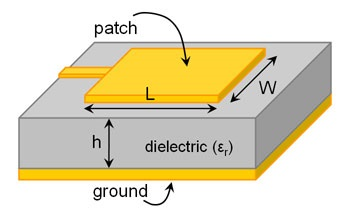
\includegraphics[width=0.4\linewidth]{img/img1}
		\caption{Structure of a Patch Antenna}
		\label{fig:img1}
	\end{figure}
	
	As mentioned above, we can see the patch antenna as a microstrip line of $L_p$ length and $W_p$ thickness, in particular: 
	\begin{equation}
		L_p=m\frac{\lambda}{2}
	\end{equation} 
	and 
	\begin{equation}
		W_p=\frac{c}{2f_r}\sqrt{\frac{2}{\varepsilon_r+1}}
		\label{Wp}
	\end{equation}
	where: 
	\begin{itemize}
		\item $\lambda$ is the wavelength 
		\item $c=3 \cdot 10^8 m/s$ is the speed of light
		\item $f_r$ is the resonance frequency of the antenna
		\item $\varepsilon_r$ is the dielectric constant of the substrate material, in our case is FR4
		
	\end{itemize}
	\subsection{Fringing effect} 
	The resonance condition for a patch antenna is typically given by \( L = \frac{\lambda}{2} \). However, as we can see in the figure below, due to edge effects, the actual path length is slightly longer, with a variation \( \Delta L \).
	\begin{figure}[h]
		\centering
		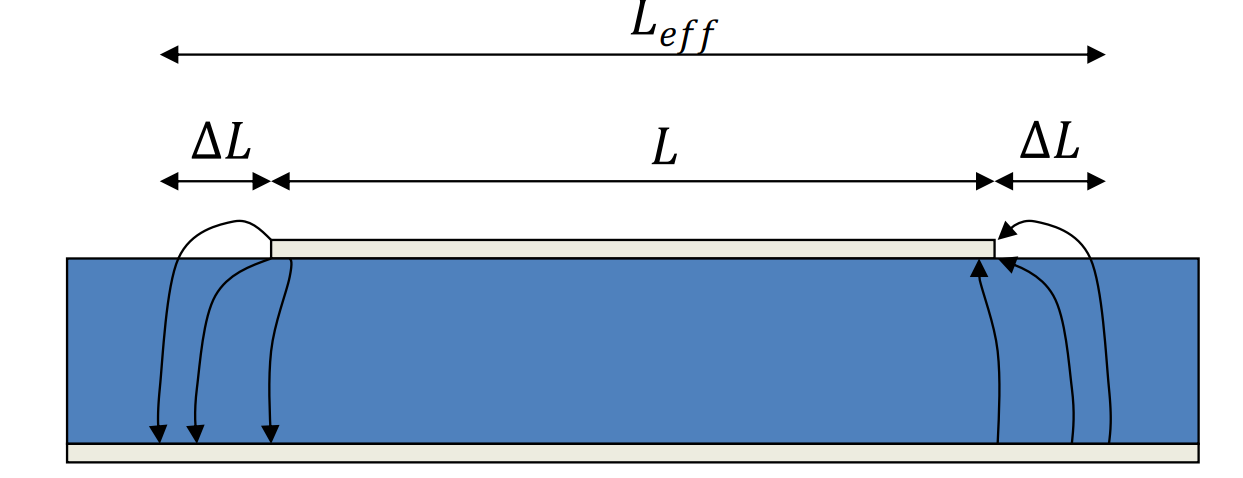
\includegraphics[width=0.4\linewidth]{img/img2}
		\caption{The electric field lines curve at the edges, increasing the electric length of the patch.}
		\label{fig:img2}
	\end{figure}
	
	
	These fringing effects cause the patch to appear longer to electromagnetic waves, leading to the definition of an effective length \( L_{\text{eff}} \) defined as: 
	\begin{equation}
		L_{eff}= L+2\Delta L
	\end{equation}
	\newpage
	where $\Delta L$ is derived from an empirical formula:
	\begin{equation}
		\Delta L \simeq h \cdot 0.412 \frac{\left( \varepsilon_\text{eff} + 0.3 \right) \left( \frac{W_p}{h} + 0.264 \right)}{\left( \varepsilon_\text{eff} - 0.258 \right) \left( \frac{W_p}{h} + 0.8 \right)}
		\label{DeltaL}
	\end{equation}
	
	and where $\varepsilon_{eff}$ is the effective relative permittivity of a microstrip of width $W_p$:
	\begin{equation}
		\varepsilon_\text{eff} \simeq \frac{\varepsilon_r + 1}{2} + \frac{\varepsilon_r - 1}{2} \frac{1}{\sqrt{1 + 12 \frac{h}{W_p}}}
		\label{Epsilon_eff}
	\end{equation}
	
	By imposing $L_\text{eff} = \frac{\lambda}{2}$ and knowing that $\lambda = \frac{c}{\sqrt{\varepsilon_\text{eff}} f_r}$, it follows that:
	\begin{equation}
		L_p = \frac{c}{2 f_r \sqrt{\varepsilon_\text{eff}}} - 2 \Delta L
		\label{Lp}
	\end{equation}
	\subsection{Impedance matching}
When designing a patch antenna, it is essential to achieve impedance matching between the feed and the characteristic impedance of the transmission line, which is typically 50~$\Omega$. This ensures optimal power transfer from the transmission line to the standing wave generated on the patch. It is not feasible to feed the patch at one edge, as the input impedance $R_i(0)$ exceeds 50~$\Omega$. The connection between the patch and the feeding line is located within the patch.

To optimize the impedance matching, the length $L$ should first be varied until an input reactance of zero is achieved at the desired resonance frequency. Following this, adjust the feed position $x_0$ to make the real part of the input impedance equal to 50~$\Omega$ at the same frequency. This process minimizes reflection and maximizes efficiency.\\
In order to achieve this value we have to exploit this formula: 
\begin{equation}
	R_i(x_0)=\frac{1}{2G_1}cos^2(\frac{\pi}{L}x_0)
	\label{R_i(x0)}
\end{equation}
	where: 
	\begin{equation}
		G_1=\frac{W_m}{120 \lambda_0}(1-\frac{1}{24}(\frac{2 \pi h}{\lambda_0})^2)
		\label{G_1}
	\end{equation}
	and 
	\begin{equation}
		\lambda_0=\frac{c}{f_r}
	\end{equation}
	
	So, by using the the \eqref{R_i(x0)} and isolate the $x_0$ term ,we are able to find the value of the feeding line slot in order to have the impedance of 50 $\Omega$, having a final result similar to the image below. 
	\begin{figure}[h]
		\centering
		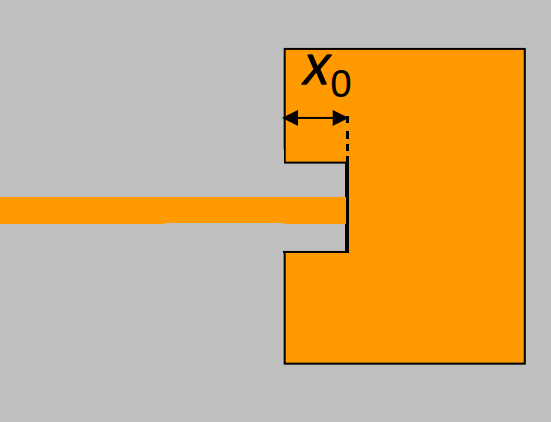
\includegraphics[width=0.4\linewidth]{img/img3}
		\caption{patch antenna with the two slot of lenght $x_0$ in orer to have the fedding line matched}
		\label{fig:img3}
	\end{figure}
	\newpage
	\section{DESIGN OF THE PATCH ANTENNA}
	\subsection{Substrate and Ground plane size}
	As previously stated, the patch antenna will be mounted on an FR4 material substrate, with a ground plane situated behind it. The initial step is to calculate the dimensions of the board using the following formula:
	\begin{equation}
		W_s=\frac{c}{f_0 \sqrt{\varepsilon_r}}
		\label{Ws}
	\end{equation}
	As can be seen, we need to know the value of $\varepsilon_r$, which is provided in the initial specifications and is equal to:
	\begin{equation}
		\varepsilon_r = 4.1 \cdot (3/f[\text{GHz}])^{0.025}
		\label{epsilon_r}
	\end{equation}
	By substituting with our value of frequency in \eqref{epsilon_r} we obtain \[\varepsilon_r = 4.1 \cdot (3/2.6[\text{GHz}])^{0.025}=4.11\] 
	so we can now substitute this value in the formula of $W_s$ \eqref{Ws}, but since we are gonna use a square board it will be: \[W_s=L_s=\frac{c}{f_0 \sqrt{\varepsilon_r}}=\frac{3 \cdot 10^8}{2.6 \cdot 10^9\sqrt{4.11}}=0,056882559 m \simeq 56.9\ mm \]
So, now we have the dimensions of the ground plane.
\subsection{Patch size}
In regard to the dimensions of the patch antenna, the width $W_p$ will be calculated using the designated formula \eqref{Wp}, so: 
\[W_p=\frac{3 \cdot 10^8}{2 \cdot 2.6 \cdot 10^9}\sqrt{\frac{2}{4.11+1}}=0,03607639
 \simeq 36.1 \ mm\]
For the length $L_p$, the formula \eqref{Lp} will be employed, with consideration for fringing effects, so first of all we have to determine the value of $\Delta L$, but before doing that we have to calculate the value of $\varepsilon_{eff}$ using the equation \eqref{Epsilon_eff}:
\[\varepsilon_\text{eff} \simeq \frac{4.11 + 1}{2} + \frac{4.11 - 1}{2} \frac{1}{\sqrt{1 + 12 \frac{1.6 \cdot 10^{-3}}{36.1 \cdot 10^{-3}}}}=3,811381 \simeq 3,81\]
so we can now calculate the value of $\Delta L$, by put all the value in the formula \eqref{DeltaL}:
\[	\Delta L \simeq 1.6 \cdot 10^{-3} \cdot 0.412 \frac{\left( 3.81 + 0.3 \right) \left( \frac{36.1 \cdot 10^{-3}}{1.6\cdot 10^{-3}} + 0.264 \right)}{\left( 3.81 - 0.258 \right) \left( \frac{36.1\cdot 10^{-3}}{1.6 \cdot 10^{-3}} + 0.8 \right)} = 0,00074509
\ m \simeq 0.745 \ mm
\]

so, finally we can calculate the value of $L_p$, let's substitute all the value in \eqref{Lp}: 
\[L_p = \frac{3 \cdot 10^8}{2\cdot 2.6 \cdot 10^9 \sqrt{3.81}} - 2\cdot 0.745 \cdot 10^{-3} = 0,02804 \ m \simeq 28.0 \ mm
 \]
  Subsequent to these preliminary calculations, the creation of the substrate may be initiated, with FR4 selected as the material and the various physical values given technical specifications. The subsequent steps involve the creation of the ground plane and the design of the patch, with copper chosen as the material for the latter two layers.
 \newpage
 \subsection{Microstrip design}
 After the creation of the substrate and the patch, the microstrip will be created; this should have a characteristic line impedance as close as possible to 50 $\Omega$.
 To achieve this result, we used a macro from CST, the Impedance calculation selecting the ‘thick microstrip’ and by putting all our values we start searching for which width of the microstrip would give us an impedance value of 50 $\Omega$, in our case a value of 3.2 mm was chosen as width.
 In the figure below, you can see the use of the macro and note that with the thickness of 3.2 mm, the line impedance is approximately 49.7 ohms.
\begin{figure}[h]
	\centering
	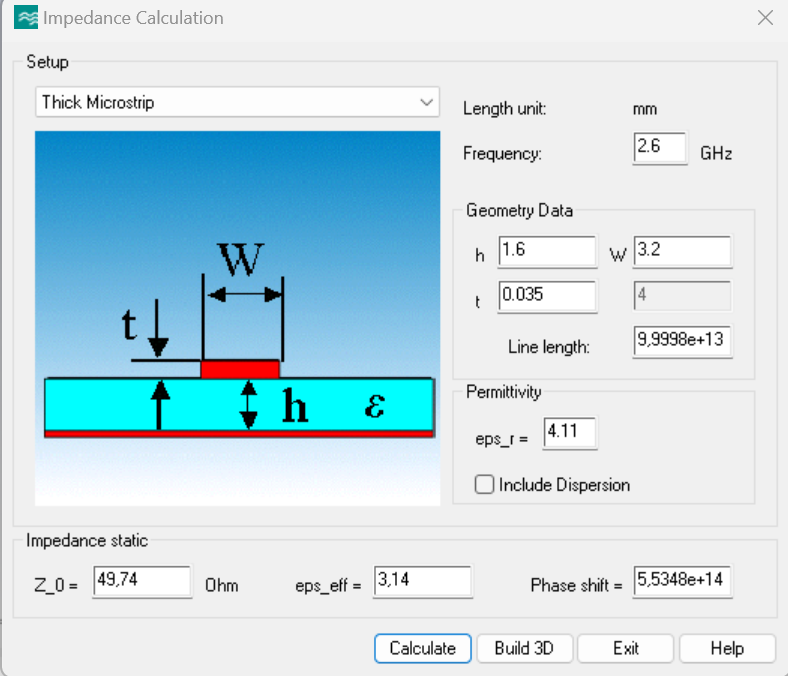
\includegraphics[width=0.4\linewidth]{img/img4}
	\caption{Macro impedance calulcation window of CST}
	\label{fig:img4}
\end{figure}

 \subsubsection{Slots design and impedance matching}
 After an initial simulation (the discussion of the results is deferred to the next section), it was necessary to introduce slots on the microstrip in order to improve antenna performance. This intervention made it possible to electrically extend the length of the microstrip, feeding the patch more internally and increasing the impedance seen at the patch input.\\
 In order to find how deep this slot must be, equation 6 was used by isolating $x_0$, obtaining: 
 \begin{equation}
 	x_0 = \frac{L}{\pi} \arccos\left(\sqrt{2G_1 R_i(x_0)}\right)
 	\label{x0}
 \end{equation}
 where, by substituting the value in \eqref{G_1} we have:
 \[
 G_1=\frac{W}{120 \cdot 115.38 \cdot 10^{-3}
  }\left[ 1-\frac{1}{24}(\frac{2 \pi 1.6\cdot 10^{-3}}{ 115.38 \cdot 10^{-3}})^2\right] = 0.002604694 \simeq 0.0026  
 \]
 so, put the value in \eqref{x0} and obtain: 
 \[
 x_0 = \frac{14.4 \cdot 10^{-3}}{\pi} \arccos\left(\sqrt{2 \cdot 0.0026 \cdot  50}\right) =  0.009241228 \simeq 9.2 \ mm
 \]
	%FINE DOCUMENTO
\end{document}